% !TeX program = xelatex
% !TeX encoding = UTF-8 Unicode
% !BIB program = biber

\documentclass{relatorio}
\usepackage[hidelinks]{hyperref}
\cftsetindents{section}{1em}{2.5em}
\cftsetindents{subsection}{1em}{5em}
\usepackage{listings}
\usepackage{parcolumns}
\usepackage{graphicx, subcaption}
\title{Is Software Debloating Useful? - A Comparative Study}
\addauthor{Sumit Lahiri}
\addauthor{Amit Kumar Sharma}
\setsubject{Analysis Study \& Comparision of Software Debloating Tools}
\preamble{}

\begin{document}
	
	\onecolumn
	\tableofcontents
	\twocolumn  
	% !TeX root = document.tex
% !TeX encoding = UTF-8 Unicode

\IEEEtitleabstractindextext{%
	\begin{abstract}
		What is Program Debloating? What is Program Debloating? What is Program Debloating? What is Program Debloating? What is Program Debloating? 
		What is Program Debloating? What is Program Debloating? What is Program Debloating? What is Program Debloating? 
		What is Program Debloating? What is Program Debloating? What is Program Debloating? What is Program Debloating? What is Program Debloating? What is Program Debloating? 
		What is Program Debloating? What is Program Debloating? What is Program Debloating? 
		What is Program Debloating? What is Program Debloating? What is Program Debloating? What is Program Debloating? What is Program Debloating? What is Program Debloating? 
		What is Program Debloating? What is Program Debloating? What is Program Debloating? What is Program Debloating? What is Program Debloating? What is Program Debloating? What is Program Debloating? What is Program Debloating? What is Program Debloating? What is Program Debloating? What is Program Debloating? What is Program Debloating? What is Program Debloating? What is Program Debloating? What is Program Debloating? What is Program Debloating? What is Program Debloating? 
	\end{abstract}
	
	\begin{IEEEkeywords}
		Software Debloating, Software Engineering, Delta Debugging
	\end{IEEEkeywords}
}

	\maketitle{}

\section{Project Objective}%
\label{Tools}

Program debloating techniques. Program deblaoting techniques rogram debloating techniques. Program deblaoting techniques
rogram debloating techniques. Program deblaoting techniquesrogram debloating techniques. Program deblaoting techniques
rogram debloating techniques. Program deblaoting techniques rogram debloating techniques. Program deblaoting techniques
rogram debloating techniques. Program deblaoting techniques 
rogram debloating techniques. Program deblaoting techniquesrogram debloating techniques. Program deblaoting techniques
rogram debloating techniques. Program deblaoting techniques

Program debloating techniques. Program deblaoting techniques rogram debloating techniques. Program deblaoting techniques
rogram debloating techniques. Program deblaoting techniquesrogram debloating techniques. Program deblaoting techniques
rogram debloating techniques. Program deblaoting techniques rogram debloating techniques. Program deblaoting techniques
rogram debloating techniques. Program deblaoting techniques 
rogram debloating techniques. Program deblaoting techniquesrogram debloating techniques. Program deblaoting techniques
rogram debloating techniques. Program deblaoting techniques

	\begin{figure}[H]
		\centering
		\captionsetup{justification=centering}
		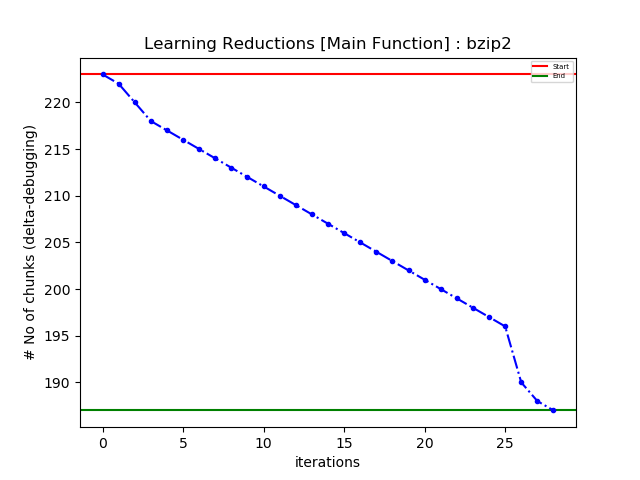
\includegraphics[width=0.65\linewidth]{imgs/chisel_learning_mkdir_plot.png}
		\caption{Learning plot for \color{blue} mkdir}%
		\label{fig:plant}
		\centering
		\captionsetup{justification=centering}
		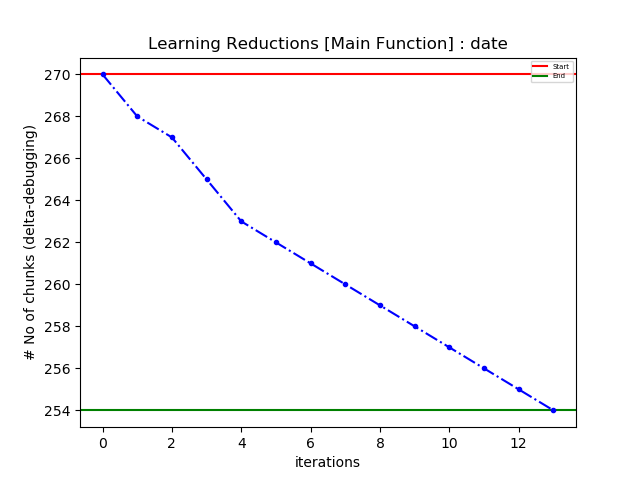
\includegraphics[width=0.65\linewidth]{imgs/chisel_learning_date_plot.png}
		\caption{Learning plot for \color{blue} date}%
		\label{fig:plant}
		\centering
		\captionsetup{justification=centering}
		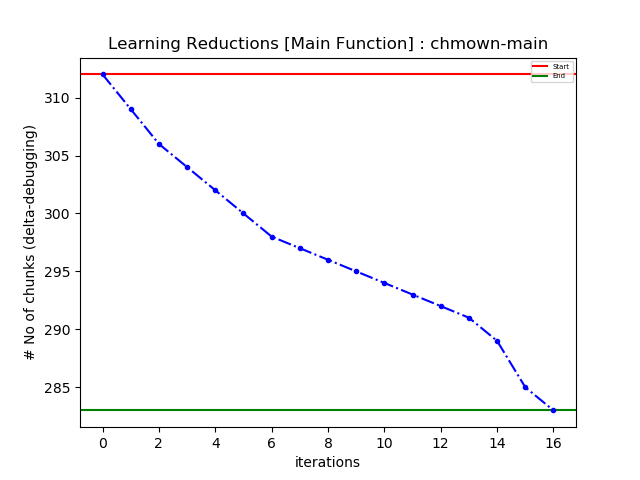
\includegraphics[width=0.65\linewidth]{imgs/chisel_learning_chmown-main_plot.png}
		\caption{Learning plot for \color{blue} chown}%
		\label{fig:plant}
		\centering
		\captionsetup{justification=centering}
		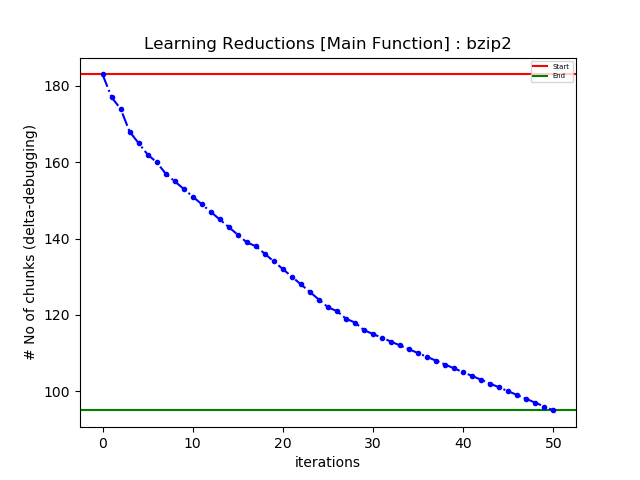
\includegraphics[width=0.65\linewidth]{imgs/chisel_learning_bzip2_plot.png}
		\caption{Learning plot for \color{blue} bzip2}%
		\label{fig:plant}
		\centering
		\captionsetup{justification=centering}
		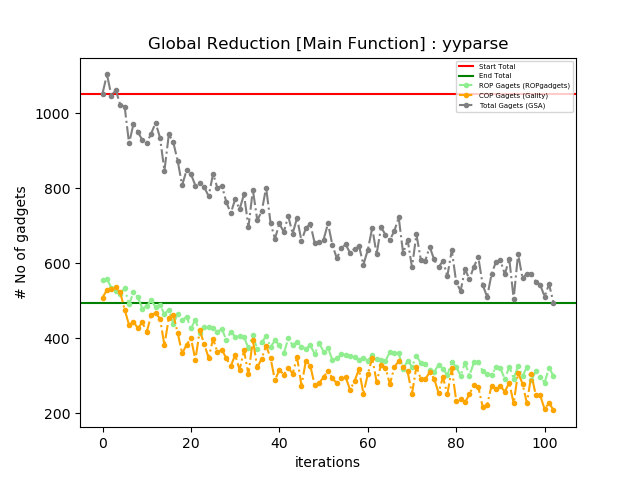
\includegraphics[width=0.65\linewidth]{imgs/chisel_gadgets_yyparse_plot.png}
		\caption{Gadgets plot for \color{blue} yyparse}%
		\label{fig:plant}
	\end{figure}
	\begin{figure}[H]
		\centering
		\captionsetup{justification=centering}
		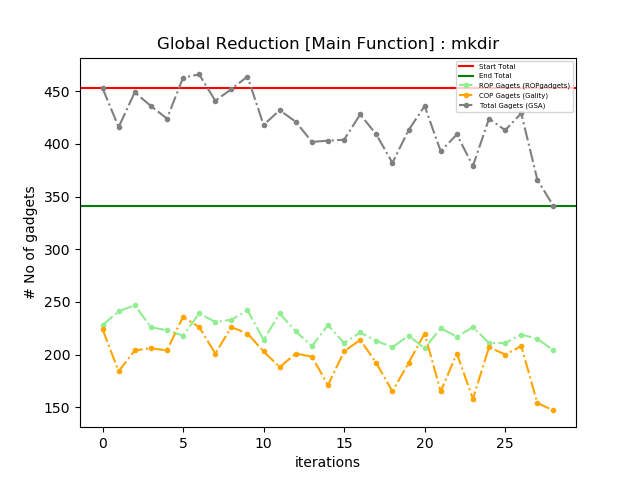
\includegraphics[width=0.65\linewidth]{imgs/chisel_gadgets_mkdir_plot.png}
		\caption{Gadgets plot for \color{blue} mkdir}%
		\label{fig:plant}
		\centering
		\captionsetup{justification=centering}
		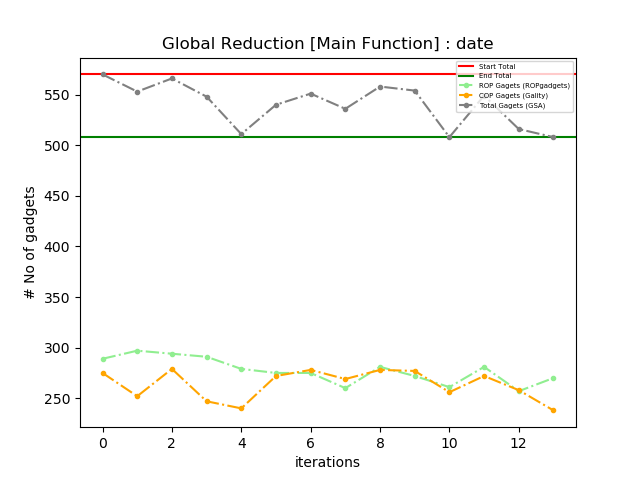
\includegraphics[width=0.65\linewidth]{imgs/chisel_gadgets_date_plot.png}
		\caption{Gadgets plot for \color{blue} date}%
		\label{fig:plant}
		\centering
		\captionsetup{justification=centering}
		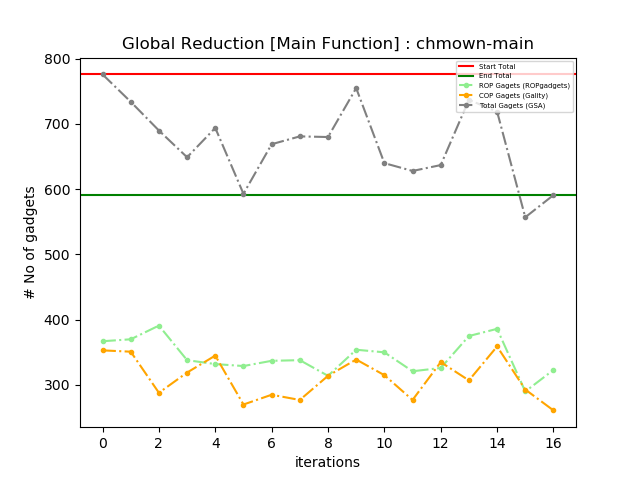
\includegraphics[width=0.65\linewidth]{imgs/chisel_gadgets_chmown-main_plot.png}
		\caption{Gadgets plot for \color{blue} chown}%
		\label{fig:plant}
		\centering
		\captionsetup{justification=centering}
		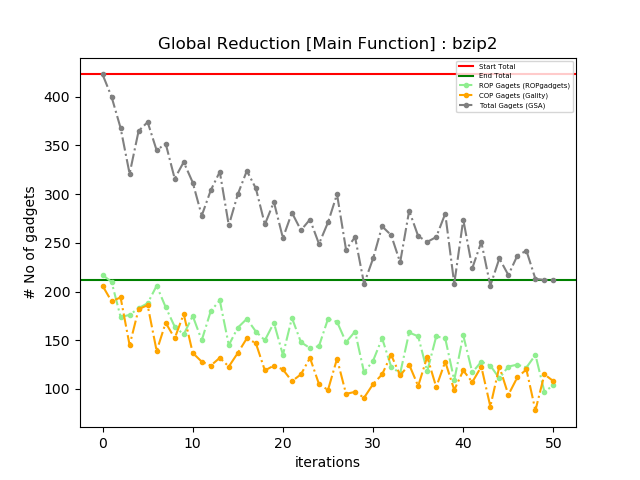
\includegraphics[width=0.65\linewidth]{imgs/chisel_gadgets_bzip2_plot.png}
		\caption{Gadgets plot for \color{blue} bzip2}%
		\label{fig:plant}
		\centering
		\captionsetup{justification=centering}
		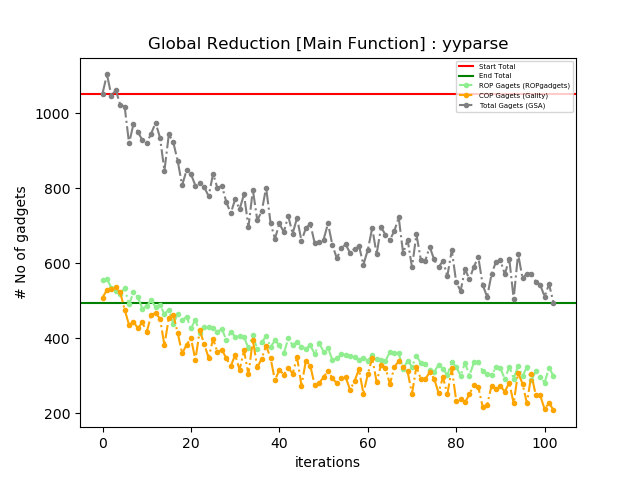
\includegraphics[width=0.65\linewidth]{imgs/chisel_gadgets_yyparse_plot.png}
		\caption{Gadgets plot for \color{blue} yyparse}%
		\label{fig:plant}
	\end{figure}


\section{What is Software debloating?}%
\label{Tools}

Program debloating techniques. Program deblaoting techniques rogram debloating techniques. Program deblaoting techniques
rogram debloating techniques. Program deblaoting techniquesrogram debloating techniques. Program deblaoting techniques
rogram debloating techniques. Program deblaoting techniques rogram debloating techniques. Program deblaoting techniques
rogram debloating techniques. Program deblaoting techniques 
rogram debloating techniques. Program deblaoting techniquesrogram debloating techniques. Program deblaoting techniques
rogram debloating techniques. Program deblaoting techniques

Program debloating techniques. Program deblaoting techniques rogram debloating techniques. Program deblaoting techniques
rogram debloating techniques. Program deblaoting techniquesrogram debloating techniques. Program deblaoting techniques
rogram debloating techniques. Program deblaoting techniques rogram debloating techniques. Program deblaoting techniques
rogram debloating techniques. Program deblaoting techniques 
rogram debloating techniques. Program deblaoting techniquesrogram debloating techniques. Program deblaoting techniques
rogram debloating techniques. Program deblaoting techniques

\subsection{Software Debloating Tools}%
\label{Tools}

Program debloating techniques. Program deblaoting techniques rogram debloating techniques. Program deblaoting techniques
rogram debloating techniques. Program deblaoting techniquesrogram debloating techniques. Program deblaoting techniques
rogram debloating techniques. Program deblaoting techniques rogram debloating techniques. Program deblaoting techniques
rogram debloating techniques. Program deblaoting techniques 
rogram debloating techniques. Program deblaoting techniquesrogram debloating techniques. Program deblaoting techniques
rogram debloating techniques. Program deblaoting techniques

Program debloating techniques. Program deblaoting techniques rogram debloating techniques. Program deblaoting techniques
rogram debloating techniques. Program deblaoting techniquesrogram debloating techniques. Program deblaoting techniques
rogram debloating techniques. Program deblaoting techniques rogram debloating techniques. Program deblaoting techniques
rogram debloating techniques. Program deblaoting techniques 
rogram debloating techniques. Program deblaoting techniquesrogram debloating techniques. Program deblaoting techniques
rogram debloating techniques. Program deblaoting techniques

\subsection{Software Debloating Techniques}%
\label{Tools}

Program debloating techniques. Program deblaoting techniques rogram debloating techniques. Program deblaoting techniques
rogram debloating techniques. Program deblaoting techniquesrogram debloating techniques. Program deblaoting techniques
rogram debloating techniques. Program deblaoting techniques rogram debloating techniques. Program deblaoting techniques
rogram debloating techniques. Program deblaoting techniques 
rogram debloating techniques. Program deblaoting techniquesrogram debloating techniques. Program deblaoting techniques
rogram debloating techniques. Program deblaoting techniques

Program debloating techniques. Program deblaoting techniques rogram debloating techniques. Program deblaoting techniques
rogram debloating techniques. Program deblaoting techniquesrogram debloating techniques. Program deblaoting techniques
rogram debloating techniques. Program deblaoting techniques rogram debloating techniques. Program deblaoting techniques
rogram debloating techniques. Program deblaoting techniques 
rogram debloating techniques. Program deblaoting techniquesrogram debloating techniques. Program deblaoting techniques
rogram debloating techniques. Program deblaoting techniques

\section{Motivating Examples}%
\label{Tools}

Program debloating techniques. Program deblaoting techniques rogram debloating techniques. Program deblaoting techniques
rogram debloating techniques. Program deblaoting techniquesrogram debloating techniques. Program deblaoting techniques
rogram debloating techniques. Program deblaoting techniques rogram debloating techniques. Program deblaoting techniques
rogram debloating techniques. Program deblaoting techniques 
rogram debloating techniques. Program deblaoting techniquesrogram debloating techniques. Program deblaoting techniques
rogram debloating techniques. Program deblaoting techniques

Program debloating techniques. Program deblaoting techniques rogram debloating techniques. Program deblaoting techniques
rogram debloating techniques. Program deblaoting techniquesrogram debloating techniques. Program deblaoting techniques
rogram debloating techniques. Program deblaoting techniques rogram debloating techniques. Program deblaoting techniques
rogram debloating techniques. Program deblaoting techniques 
rogram debloating techniques. Program deblaoting techniquesrogram debloating techniques. Program deblaoting techniques
rogram debloating techniques. Program deblaoting techniques

\section{OCCAM Tool}%
\label{Tools}

Program debloating techniques. Program deblaoting techniques rogram debloating techniques. Program deblaoting techniques
rogram debloating techniques. Program deblaoting techniquesrogram debloating techniques. Program deblaoting techniques
rogram debloating techniques. Program deblaoting techniques rogram debloating techniques. Program deblaoting techniques
rogram debloating techniques. Program deblaoting techniques 
rogram debloating techniques. Program deblaoting techniquesrogram debloating techniques. Program deblaoting techniques
rogram debloating techniques. Program deblaoting techniques

Program debloating techniques. Program deblaoting techniques rogram debloating techniques. Program deblaoting techniques
rogram debloating techniques. Program deblaoting techniquesrogram debloating techniques. Program deblaoting techniques
rogram debloating techniques. Program deblaoting techniques rogram debloating techniques. Program deblaoting techniques
rogram debloating techniques. Program deblaoting techniques 
rogram debloating techniques. Program deblaoting techniquesrogram debloating techniques. Program deblaoting techniques
rogram debloating techniques. Program deblaoting techniques

\subsection{Overview}%
\label{Tools}

Program debloating techniques. Program deblaoting techniques rogram debloating techniques. Program deblaoting techniques
rogram debloating techniques. Program deblaoting techniquesrogram debloating techniques. Program deblaoting techniques
rogram debloating techniques. Program deblaoting techniques rogram debloating techniques. Program deblaoting techniques
rogram debloating techniques. Program deblaoting techniques 
rogram debloating techniques. Program deblaoting techniquesrogram debloating techniques. Program deblaoting techniques
rogram debloating techniques. Program deblaoting techniques

Program debloating techniques. Program deblaoting techniques rogram debloating techniques. Program deblaoting techniques
rogram debloating techniques. Program deblaoting techniquesrogram debloating techniques. Program deblaoting techniques
rogram debloating techniques. Program deblaoting techniques rogram debloating techniques. Program deblaoting techniques
rogram debloating techniques. Program deblaoting techniques 
rogram debloating techniques. Program deblaoting techniquesrogram debloating techniques. Program deblaoting techniques
rogram debloating techniques. Program deblaoting techniques


\begin{table*}[]
	\begin{tabular}{lccccccc}
		\hline
		\multicolumn{8}{c}{\textbf{airtun\_ng-airtun-ng}}                                                                                                                                                                                                                                                                                                                                                                                                                                                                                                                           \\ \hline
		\multicolumn{1}{l|}{\textbf{Libraries/Tools}}                                                                                  & \multicolumn{1}{c|}{\textbf{Before}} & \multicolumn{1}{c|}{\textbf{None}} & \multicolumn{1}{c|}{\textbf{Aggressive}} & \multicolumn{1}{c|}{{\color[HTML]{CB0000} \textbf{\begin{tabular}[c]{@{}c@{}}DeepOCCAM  \\ RL Model\end{tabular}}}} & \multicolumn{1}{c|}{\textbf{\begin{tabular}[c]{@{}c@{}}Non-rec \\ Aggressive\end{tabular}}} & \multicolumn{1}{c|}{\textbf{Only once}} & {\color[HTML]{32CB00} \textbf{\begin{tabular}[c]{@{}c@{}}IPDSE/IPSCCP\\ Loop Unrolling\end{tabular}}} \\ \hline
		\multicolumn{1}{l|}{{\color[HTML]{032F62} \textbf{Functions}}}                                                                 & 4                                    & 4                                  & 3                                        & 3                                                                                          & 3                                                                                           & 4                                       & 3                                                                              \\
		\multicolumn{1}{l|}{{\color[HTML]{032F62} \textbf{Basic Blocks}}}                                                              & 451                                  & 445                                & 450                                      & 450                                                                                        & 450                                                                                         & 445                                     & 448                                                                            \\
		\multicolumn{1}{l|}{{\color[HTML]{032F62} \textbf{Instructions Count}}}                                                        & 2521                                 & 2481                               & 2523                                     & 2523                                                                                       & 2523                                                                                        & 2481                                    & 2523                                                                           \\
		\multicolumn{1}{l|}{{\color[HTML]{032F62} \textbf{Direct Calls}}}                                                              & 328                                  & 327                                & 330                                      & 330                                                                                        & 330                                                                                         & 327                                     & 330                                                                            \\
		\multicolumn{1}{l|}{{\color[HTML]{032F62} \textbf{External Calls}}}                                                            & 322                                  & 321                                & 326                                      & 326                                                                                        & 326                                                                                         & 321                                     & 325                                                                            \\
		\multicolumn{1}{c|}{{\color[HTML]{032F62} \textbf{\begin{tabular}[c]{@{}c@{}}Memory Instructions \\ Load/Store\end{tabular}}}} & 671                                  & 658                                & 672                                      & 672                                                                                        & 672                                                                                         & 658                                     & 675                                                                            \\ \hline
	\end{tabular}
\caption{Comparison of \texttt{DeepOCCAM} with other \texttt{OCCAM} Run settings and \texttt{OCCAM-T Run (Trimmer)}}
\end{table*}
\begin{table*}[]
	\begin{tabular}{lccccccc}
		\hline
		\multicolumn{8}{c}{\textbf{bzip2}}                                                                                                                                                                                                                                                                                                                                                                                                                                                                                                                                          \\ \hline
		\multicolumn{1}{l|}{\textbf{Libraries/Tools}}                                                                                  & \multicolumn{1}{c|}{\textbf{Before}} & \multicolumn{1}{c|}{\textbf{None}} & \multicolumn{1}{c|}{\textbf{Aggressive}} & \multicolumn{1}{c|}{{\color[HTML]{CB0000} \textbf{\begin{tabular}[c]{@{}c@{}}DeepOCCAM  \\ RL Model\end{tabular}}}} & \multicolumn{1}{c|}{\textbf{\begin{tabular}[c]{@{}c@{}}Non-rec \\ Aggressive\end{tabular}}} & \multicolumn{1}{c|}{\textbf{Only once}} & {\color[HTML]{32CB00} \textbf{\begin{tabular}[c]{@{}c@{}}IPDSE/IPSCCP\\ Loop Unrolling\end{tabular}}} \\ \hline
		\multicolumn{1}{l|}{{\color[HTML]{032F62} \textbf{Functions}}}                                                                 & 61                                   & 35                                 & 54                                       & 54                                                                                         & 54                                                                                          & 35                                      & 54                                                                             \\
		\multicolumn{1}{l|}{{\color[HTML]{032F62} \textbf{Basic Blocks}}}                                                              & 2776                                 & 2538                               & 3137                                     & 3137                                                                                       & 3137                                                                                        & 2538                                    & 3137                                                                           \\
		\multicolumn{1}{l|}{{\color[HTML]{032F62} \textbf{Instructions Count}}}                                                        & 24412                                & 20540                              & 23769                                    & 23769                                                                                      & 23769                                                                                       & 20540                                   & 23769                                                                          \\
		\multicolumn{1}{l|}{{\color[HTML]{032F62} \textbf{Direct Calls}}}                                                              & 4714                                 & 621                                & 1011                                     & 1011                                                                                       & 1011                                                                                        & 621                                     & 1011                                                                           \\
		\multicolumn{1}{l|}{{\color[HTML]{032F62} \textbf{External Calls}}}                                                            & 4575                                 & 515                                & 835                                      & 835                                                                                        & 835                                                                                         & 515                                     & 835                                                                            \\
		\multicolumn{1}{c|}{{\color[HTML]{032F62} \textbf{\begin{tabular}[c]{@{}c@{}}Memory Instructions \\ Load/Store\end{tabular}}}} & 5144                                 & 5209                               & 5989                                     & 5989                                                                                       & 5989                                                                                        & 5209                                    & 5989                                                                           \\ \hline
	\end{tabular}
\caption{Comparison of \texttt{DeepOCCAM} with other \texttt{OCCAM} Run settings and \texttt{OCCAM-T Run (Trimmer)}}
\end{table*}
\begin{table*}[]
	\begin{tabular}{lccccccc}
		\hline
		\multicolumn{8}{c}{\textbf{curl}}                                                                                                                                                                                                                                                                                                                                                                                                                                                                                                                                                                  \\ \hline
		\multicolumn{1}{l|}{\textbf{Libraries/Tools}}                                                                                  & \multicolumn{1}{c|}{\textbf{Before}} & \multicolumn{1}{c|}{\textbf{None}} & \multicolumn{1}{c|}{\textbf{Aggressive}} & \multicolumn{1}{c|}{{\color[HTML]{CB0000} \textbf{\begin{tabular}[c]{@{}c@{}}DeepOCCAM  \\ RL Model\end{tabular}}}} & \multicolumn{1}{c|}{\textbf{\begin{tabular}[c]{@{}c@{}}Non-rec \\ Aggressive\end{tabular}}} & \multicolumn{1}{c|}{\textbf{Only once}} & {\color[HTML]{32CB00} \textbf{\begin{tabular}[c]{@{}c@{}}IPDSE/IPSCCP\\ Loop Unrolling\end{tabular}}} \\ \hline
		\multicolumn{1}{l|}{{\color[HTML]{032F62} \textbf{Functions}}}                                                                 & 124                                  & 59                                 & 62                                       & 62                                                                                         & 52                                                                                          & 59                                      & 57                                                                                                    \\
		\multicolumn{1}{l|}{{\color[HTML]{032F62} \textbf{Basic Blocks}}}                                                              & 2823                                 & 2764                               & 4256                                     & 4375                                                                                       & 3369                                                                                        & 2764                                    & 3369                                                                                                  \\
		\multicolumn{1}{l|}{{\color[HTML]{032F62} \textbf{Instructions Count}}}                                                        & 11870                                & 11777                              & 17965                                    & 18106                                                                                      & 14512                                                                                       & 11777                                   & 15854                                                                                                 \\
		\multicolumn{1}{l|}{{\color[HTML]{032F62} \textbf{Direct Calls}}}                                                              & 1786                                 & 1696                               & 2423                                     & 2500                                                                                       & 2005                                                                                        & 1696                                    & 2145                                                                                                  \\
		\multicolumn{1}{l|}{{\color[HTML]{032F62} \textbf{External Calls}}}                                                            & 1234                                 & 1250                               & 1911                                     & 1911                                                                                       & 1519                                                                                        & 1250                                    & 1975                                                                                                  \\
		\multicolumn{1}{c|}{{\color[HTML]{032F62} \textbf{\begin{tabular}[c]{@{}c@{}}Memory Instructions \\ Load/Store\end{tabular}}}} & 2503                                 & 2511                               & 3698                                     & 3858                                                                                       & 3048                                                                                        & 2511                                    & 3625                                                                                                  \\ \hline
	\end{tabular}
\caption{Comparison of \texttt{DeepOCCAM} with other \texttt{OCCAM} Run settings and \texttt{OCCAM-T Run (Trimmer)}}
\end{table*}

\subsection{Working Procedure}%
\label{Tools}

Program debloating techniques. Program deblaoting techniques rogram debloating techniques. Program deblaoting techniques
rogram debloating techniques. Program deblaoting techniquesrogram debloating techniques. Program deblaoting techniques
rogram debloating techniques. Program deblaoting techniques rogram debloating techniques. Program deblaoting techniques
rogram debloating techniques. Program deblaoting techniques 
rogram debloating techniques. Program deblaoting techniquesrogram debloating techniques. Program deblaoting techniques
rogram debloating techniques. Program deblaoting techniques

Program debloating techniques. Program deblaoting techniques rogram debloating techniques. Program deblaoting techniques
rogram debloating techniques. Program deblaoting techniquesrogram debloating techniques. Program deblaoting techniques
rogram debloating techniques. Program deblaoting techniques rogram debloating techniques. Program deblaoting techniques
rogram debloating techniques. Program deblaoting techniques 
rogram debloating techniques. Program deblaoting techniquesrogram debloating techniques. Program deblaoting techniques
rogram debloating techniques. Program deblaoting techniques

\section{Trimmer Tool}%
\label{Tools}

Program debloating techniques. Program deblaoting techniques rogram debloating techniques. Program deblaoting techniques
rogram debloating techniques. Program deblaoting techniquesrogram debloating techniques. Program deblaoting techniques
rogram debloating techniques. Program deblaoting techniques rogram debloating techniques. Program deblaoting techniques
rogram debloating techniques. Program deblaoting techniques 
rogram debloating techniques. Program deblaoting techniquesrogram debloating techniques. Program deblaoting techniques
rogram debloating techniques. Program deblaoting techniques

Program debloating techniques. Program deblaoting techniques rogram debloating techniques. Program deblaoting techniques
rogram debloating techniques. Program deblaoting techniquesrogram debloating techniques. Program deblaoting techniques
rogram debloating techniques. Program deblaoting techniques rogram debloating techniques. Program deblaoting techniques
rogram debloating techniques. Program deblaoting techniques 
rogram debloating techniques. Program deblaoting techniquesrogram debloating techniques. Program deblaoting techniques
rogram debloating techniques. Program deblaoting techniques

\subsection{Overview}%
\label{Tools}
TRIMMER tool is used to specialize the target program with respect to the user defined configuration. The configuration contains the usage context of application. Compiler transformation are included in this tool for good debloating.Inter procedural  constant propagation is used in the tool which aggressively removes the unnecessary codes. With the reduction in the unused program codes, the gadget count of the program is also reduced and helps to improve the security performance of the system. 

\begin{table*}[]
	\begin{tabular}{lccccccc}
		\hline
		\multicolumn{8}{c}{\textbf{nettest\_bsd}}                                                                                                                                                                                                                                                                                                                                                                                                                                                                                                                                                                                 \\ \hline
		\multicolumn{1}{l|}{\textbf{Libraries/Tools}}                                                                                  & \multicolumn{1}{c|}{\textbf{Before}} & \multicolumn{1}{c|}{\textbf{None}} & \multicolumn{1}{c|}{\textbf{Aggressive}} & \multicolumn{1}{c|}{{\color[HTML]{CB0000} \textbf{\begin{tabular}[c]{@{}c@{}}DeepOCCAM  \\ RL Model\end{tabular}}}} & \multicolumn{1}{c|}{\textbf{\begin{tabular}[c]{@{}c@{}}Non-rec \\ Aggressive\end{tabular}}} & \multicolumn{1}{c|}{\textbf{Only once}} & {\color[HTML]{32CB00} \textbf{\begin{tabular}[c]{@{}c@{}}IPDSE/IPSCCP\\ Loop Unrolling\end{tabular}}} \\ \hline
		\multicolumn{1}{l|}{{\color[HTML]{032F62} \textbf{Functions}}}                                                                 & 33                                   & 23                                 & 24                                       & 24                                                                                                                & 24                                                                                          & 24                                      & 24                                                                                                    \\
		\multicolumn{1}{l|}{{\color[HTML]{032F62} \textbf{Basic Blocks}}}                                                              & 979                                  & 553                                & 573                                      & 573                                                                                                               & 573                                                                                         & 573                                     & 573                                                                                                   \\
		\multicolumn{1}{l|}{{\color[HTML]{032F62} \textbf{Instructions Count}}}                                                        & 6301                                 & 3045                               & 3140                                     & 3140                                                                                                              & 3140                                                                                        & 3140                                    & 3140                                                                                                  \\
		\multicolumn{1}{l|}{{\color[HTML]{032F62} \textbf{Direct Calls}}}                                                              & 862                                  & 402                                & 412                                      & 412                                                                                                               & 412                                                                                         & 412                                     & 412                                                                                                   \\
		\multicolumn{1}{l|}{{\color[HTML]{032F62} \textbf{External Calls}}}                                                            & 794                                  & 369                                & 377                                      & 377                                                                                                               & 377                                                                                         & 377                                     & 377                                                                                                   \\
		\multicolumn{1}{c|}{{\color[HTML]{032F62} \textbf{\begin{tabular}[c]{@{}c@{}}Memory Instructions \\ Load/Store\end{tabular}}}} & 2859                                 & 1350                               & 1396                                     & 1396                                                                                                              & 1396                                                                                        & 1396                                    & 1396                                                                                                  \\ \hline
	\end{tabular}
\caption{Comparison of \texttt{DeepOCCAM} with other \texttt{OCCAM} Run settings and \texttt{OCCAM-T Run (Trimmer)}}
\end{table*}
\begin{table*}[]
	\begin{tabular}{lccccccc}
		\hline
		\multicolumn{8}{c}{\textbf{httpd}}                                                                                                                                                                                                                                                                                                                                                                                                                                                                                                                                                                                        \\ \hline
		\multicolumn{1}{l|}{\textbf{Libraries/Tools}}                                                                                  & \multicolumn{1}{c|}{\textbf{Before}} & \multicolumn{1}{c|}{\textbf{None}} & \multicolumn{1}{c|}{\textbf{Aggressive}} & \multicolumn{1}{c|}{{\color[HTML]{CB0000} \textbf{\begin{tabular}[c]{@{}c@{}}DeepOCCAM  \\ RL Model\end{tabular}}}} & \multicolumn{1}{c|}{\textbf{\begin{tabular}[c]{@{}c@{}}Non-rec \\ Aggressive\end{tabular}}} & \multicolumn{1}{c|}{\textbf{Only once}} & {\color[HTML]{32CB00} \textbf{\begin{tabular}[c]{@{}c@{}}IPDSE/IPSCCP\\ Loop Unrolling\end{tabular}}} \\ \hline
		\multicolumn{1}{l|}{{\color[HTML]{032F62} \textbf{Functions}}}                                                                 & 1083                                 & 477                                & 428                                      & 430                                                                                                               & 444                                                                                         & 416                                     & 441                                                                                                   \\
		\multicolumn{1}{l|}{{\color[HTML]{032F62} \textbf{Basic Blocks}}}                                                              & 12943                                & 11615                              & 12563                                    & 13562                                                                                                             & 12999                                                                                       & 11401                                   & 12652                                                                                                 \\
		\multicolumn{1}{l|}{{\color[HTML]{032F62} \textbf{Instructions Count}}}                                                        & 83238                                & 62428                              & 65842                                    & 66521                                                                                                             & 70773                                                                                       & 61667                                   & 65252                                                                                                 \\
		\multicolumn{1}{l|}{{\color[HTML]{032F62} \textbf{Direct Calls}}}                                                              & 22603                                & 5279                               & 5152                                     & 5259                                                                                                              & 5932                                                                                        & 5175                                    & 5869                                                                                                  \\
		\multicolumn{1}{l|}{{\color[HTML]{032F62} \textbf{External Calls}}}                                                            & 20712                                & 4152                               & 4563                                     & 4628                                                                                                              & 4787                                                                                        & 4116                                    & 4625                                                                                                  \\
		\multicolumn{1}{c|}{{\color[HTML]{032F62} \textbf{\begin{tabular}[c]{@{}c@{}}Memory Instructions \\ Load/Store\end{tabular}}}} & 17071                                & 16334                              & 18345                                    & 17056                                                                                                             & 18347                                                                                       & 16188                                   & 17854                                                                                                 \\ \hline
	\end{tabular}
\caption{Comparison of \texttt{DeepOCCAM} with other \texttt{OCCAM} Run settings and \texttt{OCCAM-T Run (Trimmer)}}
\end{table*}
\begin{table*}[]
	\begin{tabular}{lccccccc}
		\hline
		\multicolumn{8}{c}{\textbf{GNU Tree}}                                                                                                                                                                                                                                                                                                                                                                                                                                                                                                                                                                                                         \\ \hline
		\multicolumn{1}{l|}{\textbf{Libraries/Tools}}                                                                                  & \multicolumn{1}{c|}{\textbf{Before}} & \multicolumn{1}{c|}{\textbf{None}} & \multicolumn{1}{c|}{\textbf{Aggressive}} & \multicolumn{1}{c|}{{\color[HTML]{CB0000} \textbf{\begin{tabular}[c]{@{}c@{}}DeepOCCAM  \\ RL Model\end{tabular}}}} & \multicolumn{1}{c|}{\textbf{\begin{tabular}[c]{@{}c@{}}Non-rec \\ Aggressive\end{tabular}}} & \multicolumn{1}{c|}{\textbf{Only once}} & \multicolumn{1}{c}{{\color[HTML]{32CB00} \textbf{\begin{tabular}[c]{@{}c@{}}IPDSE/IPSCCP\\ Loop Unrolling\end{tabular}}}} \\ \hline
		\multicolumn{1}{l|}{{\color[HTML]{032F62} \textbf{Functions}}}                                                                 & 52                                   & 40                                 & 41                                       & 44                                                                                                                & 44                                                                                          & 40                                      & 42                                                                                                                        \\
		\multicolumn{1}{l|}{{\color[HTML]{032F62} \textbf{Basic Blocks}}}                                                              & 1458                                 & 1845                               & 1850                                     & 1891                                                                                                              & 1891                                                                                        & 1845                                    & 1850                                                                                                                      \\
		\multicolumn{1}{l|}{{\color[HTML]{032F62} \textbf{Instructions Count}}}                                                        & 7442                                 & 8957                               & 9152                                     & 9286                                                                                                              & 9286                                                                                        & 8957                                    & 9365                                                                                                                      \\
		\multicolumn{1}{l|}{{\color[HTML]{032F62} \textbf{Direct Calls}}}                                                              & 1051                                 & 1257                               & 1150                                     & 1290                                                                                                              & 1290                                                                                        & 1257                                    & 1362                                                                                                                      \\
		\multicolumn{1}{l|}{{\color[HTML]{032F62} \textbf{External Calls}}}                                                            & 845                                  & 1167                               & 1147                                     & 1200                                                                                                              & 1200                                                                                        & 1167                                    & 1058                                                                                                                      \\
		\multicolumn{1}{c|}{{\color[HTML]{032F62} \textbf{\begin{tabular}[c]{@{}c@{}}Memory Instructions \\ Load/Store\end{tabular}}}} & 1944                                 & 2362                               & 2344                                     & 2344                                                                                                              & 2344                                                                                        & 2222                                    & 2452                                                                                                                      \\ \hline
	\end{tabular}
\caption{Comparison of \texttt{DeepOCCAM} with other \texttt{OCCAM} Run settings and \texttt{OCCAM-T Run (Trimmer)}}
\end{table*}

\subsection{Working Procedure}%
\label{Tools}

The source code is converted to LLVM IR  and given as an input to the trimmer tool along with the manifest file consisting of user defined configuration. The TRIMMER first performs input specialization with respect to the user defined configuration . The second part is loop unrolling . The loop unrolling becomes important step to make interprocedural constant propagation easier. Constant Propagation is the final stage in the tool. The specialized code processed by the TRIMMER is then given as input to the linker . The linker also reads the linker flags from the manifest file and generates a final specialized binary executable file.

\section{Chisel Tool}%
\label{Tools}

Program debloating techniques. Program deblaoting techniques rogram debloating techniques. Program deblaoting techniques
rogram debloating techniques. Program deblaoting techniquesrogram debloating techniques. Program deblaoting techniques
rogram debloating techniques. Program deblaoting techniques rogram debloating techniques. Program deblaoting techniques
rogram debloating techniques. Program deblaoting techniques 
rogram debloating techniques. Program deblaoting techniquesrogram debloating techniques. Program deblaoting techniques
rogram debloating techniques. Program deblaoting techniques

Program debloating techniques. Program deblaoting techniques rogram debloating techniques. Program deblaoting techniques
rogram debloating techniques. Program deblaoting techniquesrogram debloating techniques. Program deblaoting techniques
rogram debloating techniques. Program deblaoting techniques rogram debloating techniques. Program deblaoting techniques
rogram debloating techniques. Program deblaoting techniques 
rogram debloating techniques. Program deblaoting techniquesrogram debloating techniques. Program deblaoting techniques
rogram debloating techniques. Program deblaoting techniques	

\subsection{Overview}%
\label{Tools}

CHISEL is a program debloating and optimization tool based on syntax guided hierarchical delta debugging algorithm. The tool ensures that the reduced program are compilable, core functionalities of source program are preserved  and undefined behaviours for non core functionalities does not show up. CHISEL also keeps all the criteria required for the system to work properly in order. The criteria are minimality,naturalness,efficiency,robustness and generality. The probabilistic model is used in CHISEL to accelerate the delta debugging algorithm and Markov Decision Process is used to search a proper policy for learning the machine learning algorithm. Model based Reinforcement algorithm is used to converge to the solution quickly.

\subsection{Working Procedure}%
\label{Tools}

The input to the \textbf{CHISEL} tool is a C/C++ source file (test.c) which is to be debloated. Along with the source file , we give a specialized script which contains the high level specification of the desired output. The CHISEL tool then generates binary of the source code(test.c.chisel.c). Both the source and debloated program are then compiled by g++ or any other compiler and the binaries generated by the compiler are given to the ROP gadgets or Gadget Set Analyser(GSA) . The ROP gadget outputs the count of the  gadgets before and after debloating respectively.

\subsection{State Encoding}%
\label{Tools}

Markov Decision Process is used for Delta debugging algorithm. For  delta debugging algorithm two things are required and the tuple of these two things defines the state of the model at any time. The first thing is the pair of the program to be tested and second thing is the number of partitions into which a program is broken. The initial state consist the entire program  represented as a list into two partitions. The program can be broken inti tokens,identifiers ,statements or even a finer granularity is reached to obtain the minimal state.

\subsection{Delta Debugging}%
\label{Tools}

Delta debugging is an algorithm or technique to remove the unnecessary part of the input which is not responsible for test case failure. DD makes testing easier as it divides input into smaller subsets because smaller  and simplified testcases are easy to handle. Delta debugging algorithm is used till we reach 1-minimal expression. DD is an iterative algorithm.Markov Decision Process for delta debugging is deployed to build a statistical model to get 1-minimal solution with lesser number of iterations than delta debugging alone.


\subsection{1-minimal Program}%
\label{Tools}

Suppose we have a testcase T which fails the program P. When T is given as input to P, the entire part of T may not be responsible for causing failure to the program P. Therefore, we are interested in the exact part of T which causes the program to fail. In short, we can say failing test case can have relevant and non-relevant information. To filter out the relevant information from the test case, we use Delta debugging algorithm.If a test case T fails the program P, then the expression T’ derived from T is 1-minimal iff any deviation causes the test case failure to go away.

\section{DeepOCCAM Tool}%
\label{Tools}

Program debloating techniques. Program deblaoting techniques rogram debloating techniques. Program deblaoting techniques
rogram debloating techniques. Program deblaoting techniquesrogram debloating techniques. Program deblaoting techniques
rogram debloating techniques. Program deblaoting techniques rogram debloating techniques. Program deblaoting techniques
rogram debloating techniques. Program deblaoting techniques 
rogram debloating techniques. Program deblaoting techniquesrogram debloating techniques. Program deblaoting techniques
rogram debloating techniques. Program deblaoting techniques

Program debloating techniques. Program deblaoting techniques rogram debloating techniques. Program deblaoting techniques
rogram debloating techniques. Program deblaoting techniquesrogram debloating techniques. Program deblaoting techniques
rogram debloating techniques. Program deblaoting techniques rogram debloating techniques. Program deblaoting techniques
rogram debloating techniques. Program deblaoting techniques 
rogram debloating techniques. Program deblaoting techniquesrogram debloating techniques. Program deblaoting techniques
rogram debloating techniques. Program deblaoting techniques	

\subsection{Overview}%
\label{Tools}

Program debloating techniques. Program deblaoting techniques rogram debloating techniques. Program deblaoting techniques
rogram debloating techniques. Program deblaoting techniquesrogram debloating techniques. Program deblaoting techniques
rogram debloating techniques. Program deblaoting techniques rogram debloating techniques. Program deblaoting techniques
rogram debloating techniques. Program deblaoting techniques 
rogram debloating techniques. Program deblaoting techniquesrogram debloating techniques. Program deblaoting techniques
rogram debloating techniques. Program deblaoting techniques

Program debloating techniques. Program deblaoting techniques rogram debloating techniques. Program deblaoting techniques
rogram debloating techniques. Program deblaoting techniquesrogram debloating techniques. Program deblaoting techniques
rogram debloating techniques. Program deblaoting techniques rogram debloating techniques. Program deblaoting techniques
rogram debloating techniques. Program deblaoting techniques 
rogram debloating techniques. Program deblaoting techniquesrogram debloating techniques. Program deblaoting techniques
rogram debloating techniques. Program deblaoting techniques
\begin{table*}[]
\centering
\begin{tabular}{l|lccccc}
	\hline
	{\color[HTML]{3166FF} \textbf{Bzip2 Program}}                                           & \multicolumn{1}{c|}{Original} & \multicolumn{1}{c|}{{\color[HTML]{009901} \begin{tabular}[c]{@{}c@{}}Chisel\\ Tool\end{tabular}}} & \multicolumn{1}{c|}{{\color[HTML]{3166FF} \begin{tabular}[c]{@{}c@{}}OCCAM-T\\ (Trimmer)\end{tabular}}} & \multicolumn{1}{c|}{{\color[HTML]{CB0000} \begin{tabular}[c]{@{}c@{}}DeepOCCAM\\ RL Model\end{tabular}}} & \multicolumn{1}{c|}{\begin{tabular}[c]{@{}c@{}}OCCAM\\ Aggressive\end{tabular}} & \begin{tabular}[c]{@{}c@{}}OCCAM \\ None\end{tabular} \\ \hline
	ROP Gadgets                                                                             & 646                          & 313                                                                                               & 1311                                                                                                    & 1395                                                                                                     & 1336                                                                            & 1455                                                  \\
	COP Gadgets                                                                             & 97                           & 55                                                                                                & 208                                                                                                     & 226                                                                                                      & 205                                                                             & 236                                                   \\
	JOP Gadgets                                                                             & 6872                         & 1562                                                                                              & 3784                                                                                                    & 3722                                                                                                     & 3848                                                                            & 4585                                                  \\
	\begin{tabular}[c]{@{}l@{}}Total Unique Gadgets\\ (Excluding SYS \& Chain)\end{tabular} & 7374                         & 1930                                                                                              & 5284                                                                                                    & 5117                                                                                                     & 5185                                                                            & 6345                                                  \\ \hline
\end{tabular}
	\caption{Gadgets count comparision for \color{blue} Bzip2}
\end{table*}	

\begin{table*}[]
	\centering
	\begin{tabular}{l|cccccc}
		\hline
		{\color[HTML]{3166FF} \textbf{GNU Tree}}                                                & \multicolumn{1}{c|}{Original} & \multicolumn{1}{c|}{{\color[HTML]{009901} \begin{tabular}[c]{@{}c@{}}Chisel\\ Tool\end{tabular}}} & \multicolumn{1}{c|}{{\color[HTML]{3166FF} \begin{tabular}[c]{@{}c@{}}OCCAM-T\\ (Trimmer)\end{tabular}}} & \multicolumn{1}{c|}{{\color[HTML]{CB0000} \begin{tabular}[c]{@{}c@{}}DeepOCCAM\\ RL Model\end{tabular}}} & \multicolumn{1}{c|}{\begin{tabular}[c]{@{}c@{}}OCCAM\\ Aggressive\end{tabular}} & \begin{tabular}[c]{@{}c@{}}OCCAM \\ None\end{tabular} \\ \hline
		ROP Gadgets                                                                             & 567                           & 405                                                                                               & 483                                                                                                     & 567                                                                                                      & 713                                                                             & 515                                                   \\
		COP Gadgets                                                                             & 50                            & 9                                                                                               & 19                                                                                                      & 146                                                                                                      & 39                                                                              & 83                                                    \\
		JOP Gadgets                                                                             & 2126                          & 775                                                                                              & 2774                                                                                                    & 1951                                                                                                     & 1951                                                                            & 2564                                                  \\
		\begin{tabular}[c]{@{}l@{}}Total Unique Gadgets\\ (Excluding SYS \& Chain)\end{tabular} & 2693                          & 0                                                                                              & 3258                                                                                                    & 2664                                                                                                     & 2664                                                                            & 3162                                                  \\ \hline
	\end{tabular}
	\caption{Gadgets count comparision for \color{blue} GNU Tree}
\end{table*}

\subsection{Working Procedure}%
\label{Tools}

Program debloating techniques. Program deblaoting techniques rogram debloating techniques. Program deblaoting techniques
rogram debloating techniques. Program deblaoting techniquesrogram debloating techniques. Program deblaoting techniques
rogram debloating techniques. Program deblaoting techniques rogram debloating techniques. Program deblaoting techniques
rogram debloating techniques. Program deblaoting techniques 
rogram debloating techniques. Program deblaoting techniquesrogram debloating techniques. Program deblaoting techniques
rogram debloating techniques. Program deblaoting techniques

Program debloating techniques. Program deblaoting techniques rogram debloating techniques. Program deblaoting techniques
rogram debloating techniques. Program deblaoting techniquesrogram debloating techniques. Program deblaoting techniques
rogram debloating techniques. Program deblaoting techniques rogram debloating techniques. Program deblaoting techniques
rogram debloating techniques. Program deblaoting techniques 
rogram debloating techniques. Program deblaoting techniquesrogram debloating techniques. Program deblaoting techniques
rogram debloating techniques. Program deblaoting techniques

\subsection{State Encoding}%
\label{Tools}

Program debloating techniques. Program deblaoting techniques rogram debloating techniques. Program deblaoting techniques
rogram debloating techniques. Program deblaoting techniquesrogram debloating techniques. Program deblaoting techniques
rogram debloating techniques. Program deblaoting techniques rogram debloating techniques. Program deblaoting techniques
rogram debloating techniques. Program deblaoting techniques 
rogram debloating techniques. Program deblaoting techniquesrogram debloating techniques. Program deblaoting techniques
rogram debloating techniques. Program deblaoting techniques

Program debloating techniques. Program deblaoting techniques rogram debloating techniques. Program deblaoting techniques
rogram debloating techniques. Program deblaoting techniquesrogram debloating techniques. Program deblaoting techniques
rogram debloating techniques. Program deblaoting techniques rogram debloating techniques. Program deblaoting techniques
rogram debloating techniques. Program deblaoting techniques 
rogram debloating techniques. Program deblaoting techniquesrogram debloating techniques. Program deblaoting techniques
rogram debloating techniques. Program deblaoting techniques	

\subsection{Inst2Vec Usage}%
\label{Tools}

Inst2vec  is the technique of processing the source code into the features vector for modeling the Reinforcement Learning. It follows an approach similar to skip-gram model in Natural Language Processing of pre-defined context size. The source code is first compiled into LLVM IR code. The LLVM IR is in the form of a static single assignment.As LLVM IR  is independent of machine or hardware architecture and programming language , it becomes easy to train the program embeddings.The approach is similar to word2vec model.


With the LLVM IR , the contextual flow graph (XFG)is created. XFG takes into account both the data flow and control flow of the program. With these XFGs generated from LLVM IR , the consecutive statement pairs are made of pre-defined context size . These statement pairs are then  checked for duplication. The XFGs pairs are made by constructing a dual graph with statement as nodes and removing duplicate edges. The process is then followed by removing statements of negligible presence. We get an inst2vec after subsampling of frequent pairs which can be optimized and trained. XFGs ensures that the semantics of statements are preserved.

\section{Project Aim}%
\label{Tools}

Program debloating techniques. Program deblaoting techniques rogram debloating techniques. Program deblaoting techniques
rogram debloating techniques. Program deblaoting techniquesrogram debloating techniques. Program deblaoting techniques
rogram debloating techniques. Program deblaoting techniques rogram debloating techniques. Program deblaoting techniques
rogram debloating techniques. Program deblaoting techniques 
rogram debloating techniques. Program deblaoting techniquesrogram debloating techniques. Program deblaoting techniques
rogram debloating techniques. Program deblaoting techniques

Program debloating techniques. Program deblaoting techniques rogram debloating techniques. Program deblaoting techniques
rogram debloating techniques. Program deblaoting techniquesrogram debloating techniques. Program deblaoting techniques
rogram debloating techniques. Program deblaoting techniques rogram debloating techniques. Program deblaoting techniques
rogram debloating techniques. Program deblaoting techniques 
rogram debloating techniques. Program deblaoting techniquesrogram debloating techniques. Program deblaoting techniques
rogram debloating techniques. Program deblaoting techniques

\section{Implementation}%
\label{Tools}

Program debloating techniques. Program deblaoting techniques rogram debloating techniques. Program deblaoting techniques
rogram debloating techniques. Program deblaoting techniquesrogram debloating techniques. Program deblaoting techniques
rogram debloating techniques. Program deblaoting techniques rogram debloating techniques. Program deblaoting techniques
rogram debloating techniques. Program deblaoting techniques 
rogram debloating techniques. Program deblaoting techniquesrogram debloating techniques. Program deblaoting techniques
rogram debloating techniques. Program deblaoting techniques

Program debloating techniques. Program deblaoting techniques rogram debloating techniques. Program deblaoting techniques
rogram debloating techniques. Program deblaoting techniquesrogram debloating techniques. Program deblaoting techniques
rogram debloating techniques. Program deblaoting techniques rogram debloating techniques. Program deblaoting techniques
rogram debloating techniques. Program deblaoting techniques 
rogram debloating techniques. Program deblaoting techniquesrogram debloating techniques. Program deblaoting techniques
rogram debloating techniques. Program deblaoting techniques

\section{Pipeline Setup}%
\label{Tools}

Program debloating techniques. Program deblaoting techniques rogram debloating techniques. Program deblaoting techniques
rogram debloating techniques. Program deblaoting techniquesrogram debloating techniques. Program deblaoting techniques
rogram debloating techniques. Program deblaoting techniques rogram debloating techniques. Program deblaoting techniques
rogram debloating techniques. Program deblaoting techniques 
rogram debloating techniques. Program deblaoting techniquesrogram debloating techniques. Program deblaoting techniques
rogram debloating techniques. Program deblaoting techniques

Program debloating techniques. Program deblaoting techniques rogram debloating techniques. Program deblaoting techniques
rogram debloating techniques. Program deblaoting techniquesrogram debloating techniques. Program deblaoting techniques
rogram debloating techniques. Program deblaoting techniques rogram debloating techniques. Program deblaoting techniques
rogram debloating techniques. Program deblaoting techniques 
rogram debloating techniques. Program deblaoting techniquesrogram debloating techniques. Program deblaoting techniques
rogram debloating techniques. Program deblaoting techniques

	\begin{figure}[H]
	\centering
	\captionsetup{justification=centering}
	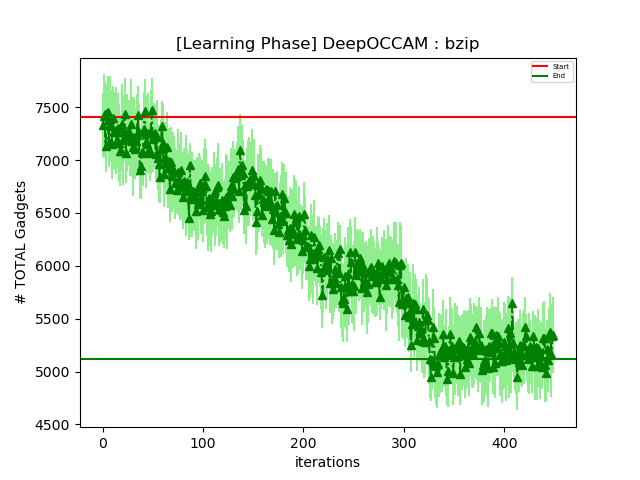
\includegraphics[width=1\linewidth]{imgs/deepoccam_HF_learning_bzip_TOTAL_plot.png}
	\caption{\textbf{DeepOCCAM} \textbf{Total} \\ \textbf{450} iterations \color{blue} bzip - HF}%
	\label{fig:plant}
	\centering
	\captionsetup{justification=centering}
	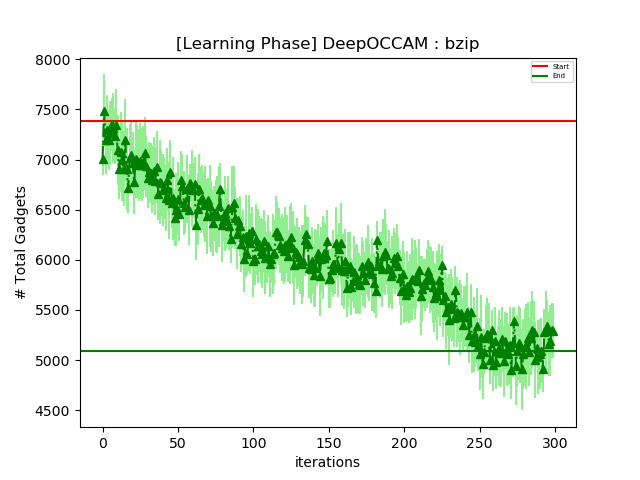
\includegraphics[width=1\linewidth]{imgs/deepoccam_inst2vec_bzip_Total_plot.png}
	\caption{\textbf{DeepOCCAM} \textbf{Total} \\ \textbf{300} iterations \color{blue} bzip - inst2vec bzip embedding}%
	\label{fig:plant}
	\centering
	\captionsetup{justification=centering}
	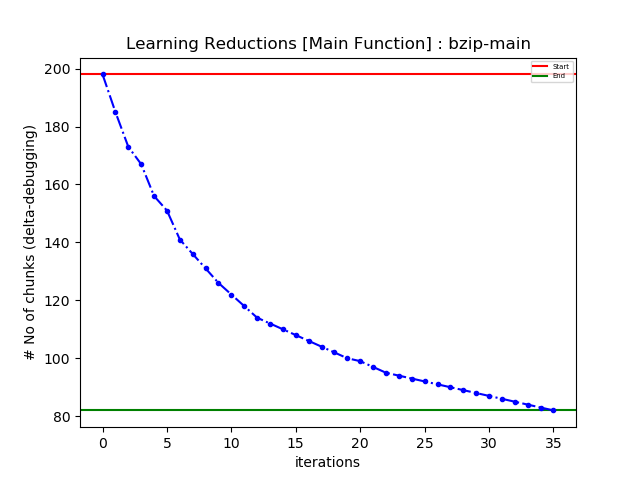
\includegraphics[width=1\linewidth]{imgs/plots/chisel_learning_bzip-main_plot.png}
	\caption{\textbf{Chisel} Learning bzip \textbf{\texttt{main()}}}%
	\label{fig:plant}
\end{figure}
\begin{figure}[H]
	\centering
	\captionsetup{justification=centering}
	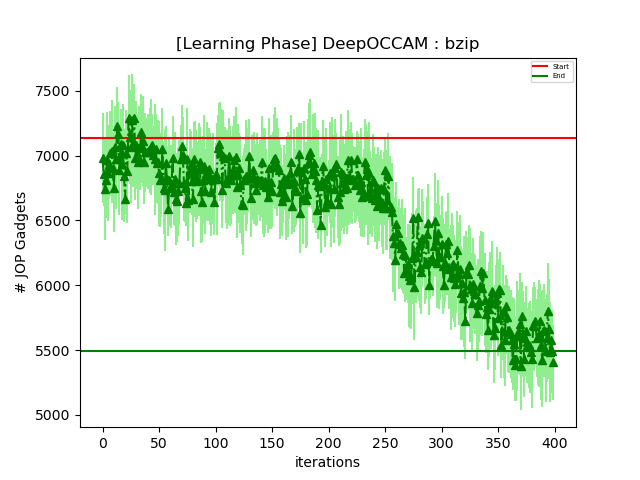
\includegraphics[width=1\linewidth]{imgs/plots/deepoccam_HF_bzip_JOP_plot.png}
	\caption{\textbf{DeepOCCAM} \textbf{JOP} \\ \textbf{400} iterations \color{blue} bzip - HF}%
	\label{fig:plant}
	\centering
	\captionsetup{justification=centering}
	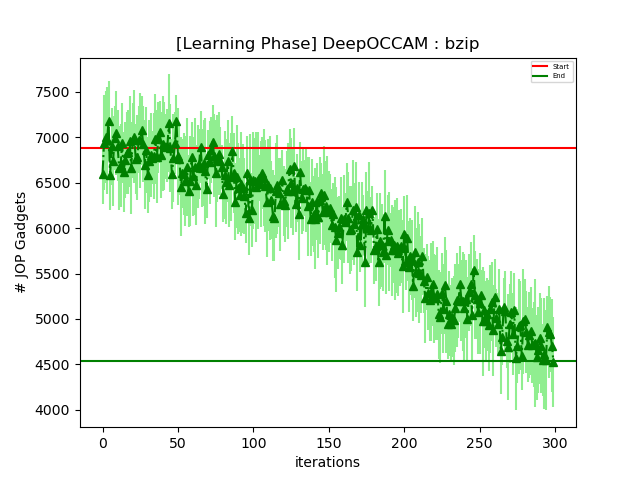
\includegraphics[width=1\linewidth]{imgs/plots/deepoccam_inst2vec_bzip_JOP_plot.png}
	\caption{\textbf{DeepOCCAM} \textbf{JOP} \\ \textbf{300} iterations \color{blue} bzip - inst2vec bzip embedding}%
	\label{fig:plant}
	\centering
	\captionsetup{justification=centering}
	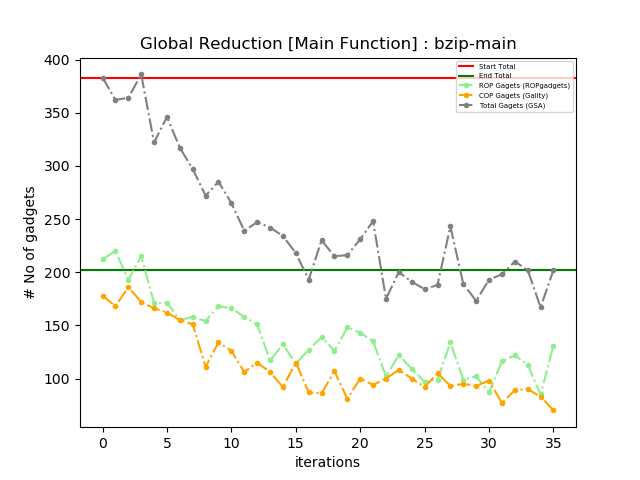
\includegraphics[width=1\linewidth]{imgs/plots/chisel_gadgets_bzip-main_plot.png}
	\caption{\textbf{Chisel} Gadgets Count \textbf{\texttt{main()}}}%
	\label{fig:plant}
\end{figure}

\subsection{Chisel Pipeline}%
\label{Tools}

Program debloating techniques. Program deblaoting techniques rogram debloating techniques. Program deblaoting techniques
rogram debloating techniques. Program deblaoting techniquesrogram debloating techniques. Program deblaoting techniques
rogram debloating techniques. Program deblaoting techniques rogram debloating techniques. Program deblaoting techniques
rogram debloating techniques. Program deblaoting techniques 
rogram debloating techniques. Program deblaoting techniquesrogram debloating techniques. Program deblaoting techniques
rogram debloating techniques. Program deblaoting techniques

Program debloating techniques. Program deblaoting techniques rogram debloating techniques. Program deblaoting techniques
rogram debloating techniques. Program deblaoting techniquesrogram debloating techniques. Program deblaoting techniques
rogram debloating techniques. Program deblaoting techniques rogram debloating techniques. Program deblaoting techniques
rogram debloating techniques. Program deblaoting techniques 
rogram debloating techniques. Program deblaoting techniquesrogram debloating techniques. Program deblaoting techniques
rogram debloating techniques. Program deblaoting techniques

\subsection{OCCAM Pipeline}%
\label{Tools}

Program debloating techniques. Program deblaoting techniques rogram debloating techniques. Program deblaoting techniques
rogram debloating techniques. Program deblaoting techniquesrogram debloating techniques. Program deblaoting techniques
rogram debloating techniques. Program deblaoting techniques rogram debloating techniques. Program deblaoting techniques
rogram debloating techniques. Program deblaoting techniques 
rogram debloating techniques. Program deblaoting techniquesrogram debloating techniques. Program deblaoting techniques
rogram debloating techniques. Program deblaoting techniques

Program debloating techniques. Program deblaoting techniques rogram debloating techniques. Program deblaoting techniques
rogram debloating techniques. Program deblaoting techniquesrogram debloating techniques. Program deblaoting techniques
rogram debloating techniques. Program deblaoting techniques rogram debloating techniques. Program deblaoting techniques
rogram debloating techniques. Program deblaoting techniques 
rogram debloating techniques. Program deblaoting techniquesrogram debloating techniques. Program deblaoting techniques
rogram debloating techniques. Program deblaoting techniques

\subsection{DeepOCCAM Pipeline}%
\label{Tools}

Program debloating techniques. Program deblaoting techniques rogram debloating techniques. Program deblaoting techniques
rogram debloating techniques. Program deblaoting techniquesrogram debloating techniques. Program deblaoting techniques
rogram debloating techniques. Program deblaoting techniques rogram debloating techniques. Program deblaoting techniques
rogram debloating techniques. Program deblaoting techniques 
rogram debloating techniques. Program deblaoting techniquesrogram debloating techniques. Program deblaoting techniques
rogram debloating techniques. Program deblaoting techniques

Program debloating techniques. Program deblaoting techniques rogram debloating techniques. Program deblaoting techniques
rogram debloating techniques. Program deblaoting techniquesrogram debloating techniques. Program deblaoting techniques
rogram debloating techniques. Program deblaoting techniques rogram debloating techniques. Program deblaoting techniques
rogram debloating techniques. Program deblaoting techniques 
rogram debloating techniques. Program deblaoting techniquesrogram debloating techniques. Program deblaoting techniques
rogram debloating techniques. Program deblaoting techniques

\section{Analysis Metrics}%
\label{Tools}

Program debloating techniques. Program deblaoting techniques rogram debloating techniques. Program deblaoting techniques
rogram debloating techniques. Program deblaoting techniquesrogram debloating techniques. Program deblaoting techniques
rogram debloating techniques. Program deblaoting techniques rogram debloating techniques. Program deblaoting techniques
rogram debloating techniques. Program deblaoting techniques 
rogram debloating techniques. Program deblaoting techniquesrogram debloating techniques. Program deblaoting techniques
rogram debloating techniques. Program deblaoting techniques

Program debloating techniques. Program deblaoting techniques rogram debloating techniques. Program deblaoting techniques
rogram debloating techniques. Program deblaoting techniquesrogram debloating techniques. Program deblaoting techniques
rogram debloating techniques. Program deblaoting techniques rogram debloating techniques. Program deblaoting techniques
rogram debloating techniques. Program deblaoting techniques 
rogram debloating techniques. Program deblaoting techniquesrogram debloating techniques. Program deblaoting techniques
rogram debloating techniques. Program deblaoting techniques

\subsection{Static Analysis}%
\label{Tools}

Program debloating techniques. Program deblaoting techniques rogram debloating techniques. Program deblaoting techniques
rogram debloating techniques. Program deblaoting techniquesrogram debloating techniques. Program deblaoting techniques
rogram debloating techniques. Program deblaoting techniques rogram debloating techniques. Program deblaoting techniques
rogram debloating techniques. Program deblaoting techniques 
rogram debloating techniques. Program deblaoting techniquesrogram debloating techniques. Program deblaoting techniques
rogram debloating techniques. Program deblaoting techniques

Program debloating techniques. Program deblaoting techniques rogram debloating techniques. Program deblaoting techniques
rogram debloating techniques. Program deblaoting techniquesrogram debloating techniques. Program deblaoting techniques
rogram debloating techniques. Program deblaoting techniques rogram debloating techniques. Program deblaoting techniques
rogram debloating techniques. Program deblaoting techniques 
rogram debloating techniques. Program deblaoting techniquesrogram debloating techniques. Program deblaoting techniques
rogram debloating techniques. Program deblaoting techniques

\subsection{Dynamic Analysis}%
\label{Tools}

Program debloating techniques. Program deblaoting techniques rogram debloating techniques. Program deblaoting techniques
rogram debloating techniques. Program deblaoting techniquesrogram debloating techniques. Program deblaoting techniques
rogram debloating techniques. Program deblaoting techniques rogram debloating techniques. Program deblaoting techniques
rogram debloating techniques. Program deblaoting techniques 
rogram debloating techniques. Program deblaoting techniquesrogram debloating techniques. Program deblaoting techniques
rogram debloating techniques. Program deblaoting techniques

Program debloating techniques. Program deblaoting techniques rogram debloating techniques. Program deblaoting techniques
rogram debloating techniques. Program deblaoting techniquesrogram debloating techniques. Program deblaoting techniques
rogram debloating techniques. Program deblaoting techniques rogram debloating techniques. Program deblaoting techniques
rogram debloating techniques. Program deblaoting techniques 
rogram debloating techniques. Program deblaoting techniquesrogram debloating techniques. Program deblaoting techniques
rogram debloating techniques. Program deblaoting techniques

\subsection{Gadgets}%
\label{Tools}

Program debloating techniques. Program deblaoting techniques rogram debloating techniques. Program deblaoting techniques
rogram debloating techniques. Program deblaoting techniquesrogram debloating techniques. Program deblaoting techniques
rogram debloating techniques. Program deblaoting techniques rogram debloating techniques. Program deblaoting techniques
rogram debloating techniques. Program deblaoting techniques 
rogram debloating techniques. Program deblaoting techniquesrogram debloating techniques. Program deblaoting techniques
rogram debloating techniques. Program deblaoting techniques

Program debloating techniques. Program deblaoting techniques rogram debloating techniques. Program deblaoting techniques
rogram debloating techniques. Program deblaoting techniquesrogram debloating techniques. Program deblaoting techniques
rogram debloating techniques. Program deblaoting techniques rogram debloating techniques. Program deblaoting techniques
rogram debloating techniques. Program deblaoting techniques 
rogram debloating techniques. Program deblaoting techniquesrogram debloating techniques. Program deblaoting techniques
rogram debloating techniques. Program deblaoting techniques

\section{Comparision Metrics}%
\label{Tools}

Program debloating techniques. Program deblaoting techniques rogram debloating techniques. Program deblaoting techniques
rogram debloating techniques. Program deblaoting techniquesrogram debloating techniques. Program deblaoting techniques
rogram debloating techniques. Program deblaoting techniques rogram debloating techniques. Program deblaoting techniques
rogram debloating techniques. Program deblaoting techniques 
rogram debloating techniques. Program deblaoting techniquesrogram debloating techniques. Program deblaoting techniques
rogram debloating techniques. Program deblaoting techniques

Program debloating techniques. Program deblaoting techniques rogram debloating techniques. Program deblaoting techniques
rogram debloating techniques. Program deblaoting techniquesrogram debloating techniques. Program deblaoting techniques
rogram debloating techniques. Program deblaoting techniques rogram debloating techniques. Program deblaoting techniques
rogram debloating techniques. Program deblaoting techniques 
rogram debloating techniques. Program deblaoting techniquesrogram debloating techniques. Program deblaoting techniques
rogram debloating techniques. Program deblaoting techniques


\subsection{Static Analysis}%
\label{Tools}

Program debloating techniques. Program deblaoting techniques rogram debloating techniques. Program deblaoting techniques
rogram debloating techniques. Program deblaoting techniquesrogram debloating techniques. Program deblaoting techniques
rogram debloating techniques. Program deblaoting techniques rogram debloating techniques. Program deblaoting techniques
rogram debloating techniques. Program deblaoting techniques 
rogram debloating techniques. Program deblaoting techniquesrogram debloating techniques. Program deblaoting techniques
rogram debloating techniques. Program deblaoting techniques

Program debloating techniques. Program deblaoting techniques rogram debloating techniques. Program deblaoting techniques
rogram debloating techniques. Program deblaoting techniquesrogram debloating techniques. Program deblaoting techniques
rogram debloating techniques. Program deblaoting techniques rogram debloating techniques. Program deblaoting techniques
rogram debloating techniques. Program deblaoting techniques 
rogram debloating techniques. Program deblaoting techniquesrogram debloating techniques. Program deblaoting techniques
rogram debloating techniques. Program deblaoting techniques



\begin{figure*}
	\centering
	\captionsetup{justification=centering}
	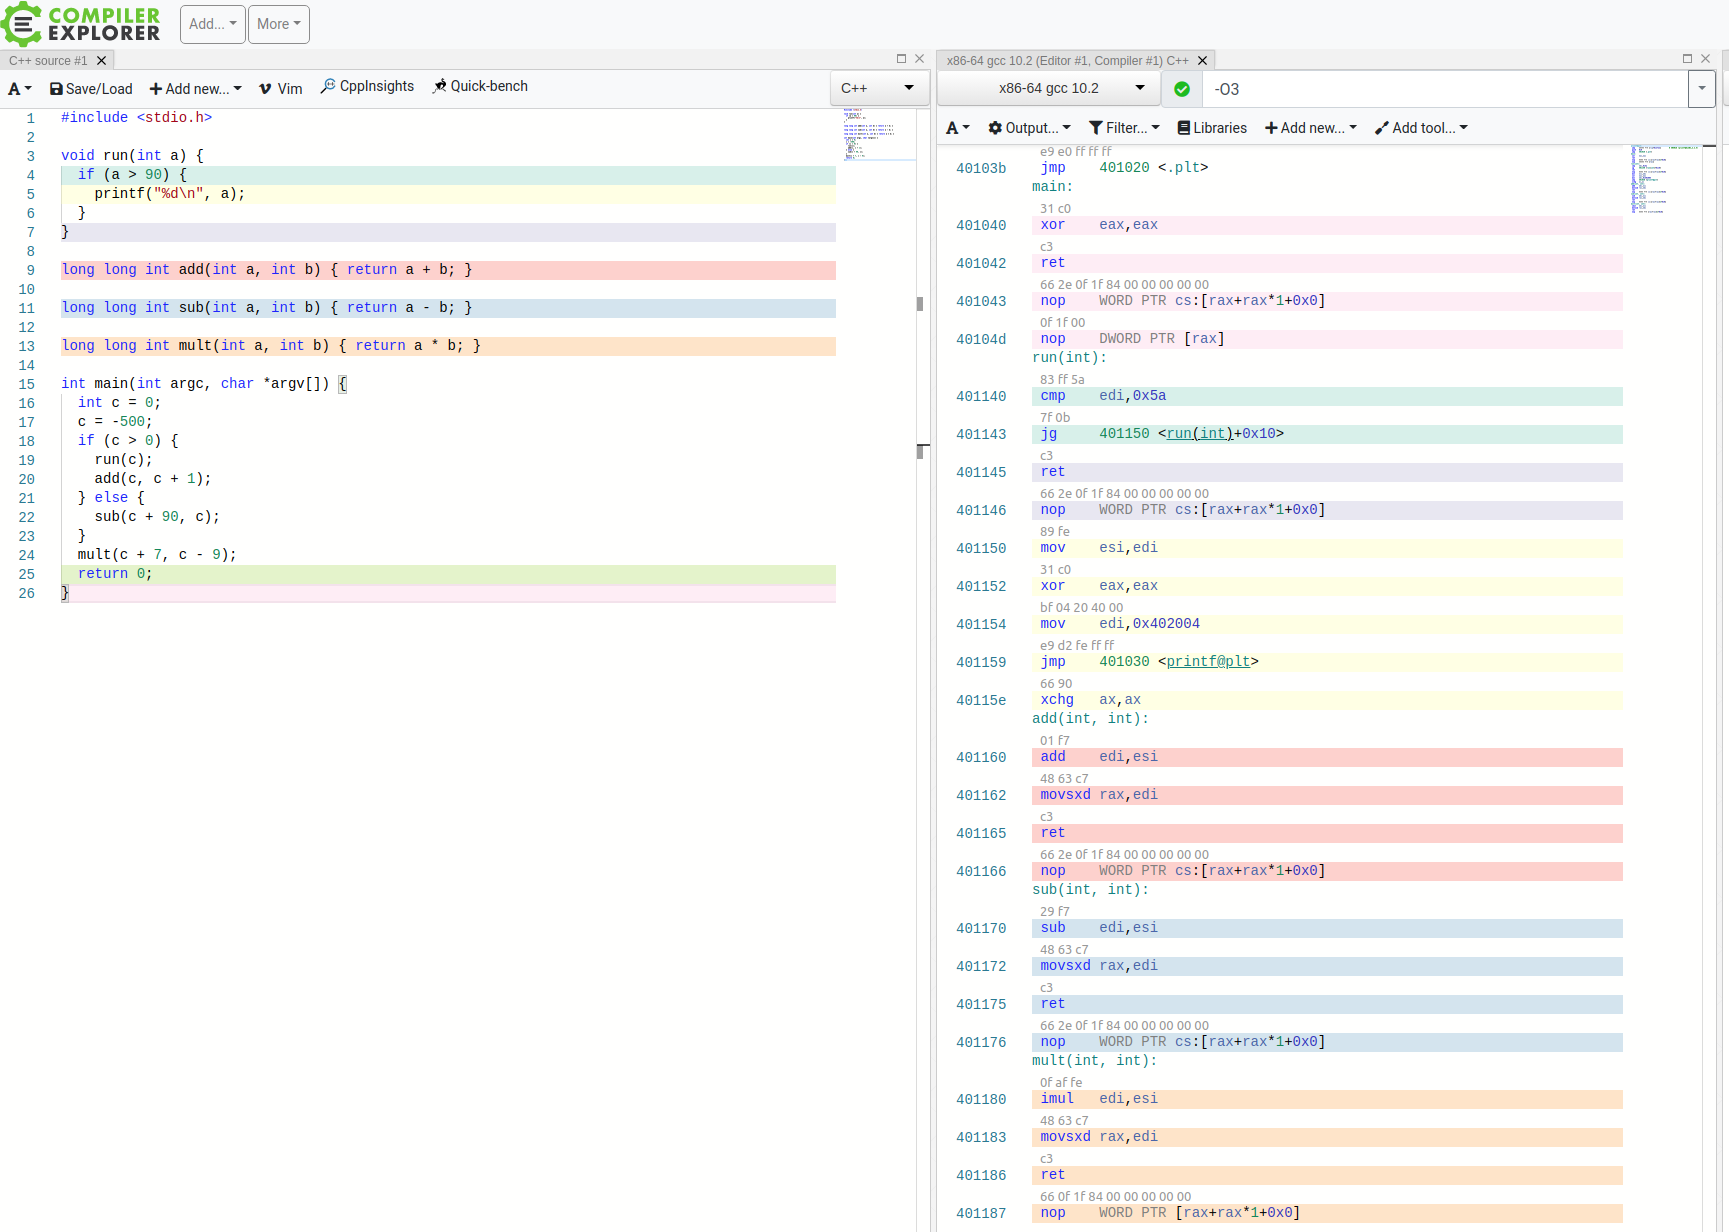
\includegraphics[width=1\linewidth]{imgs/chisel_before.png}
	\caption{\textbf{\texttt{C Code}} Example \color{red} before \color{black} \textbf{Chisel} tool processing}%
	\label{fig:plant}
	\centering
	\captionsetup{justification=centering}
	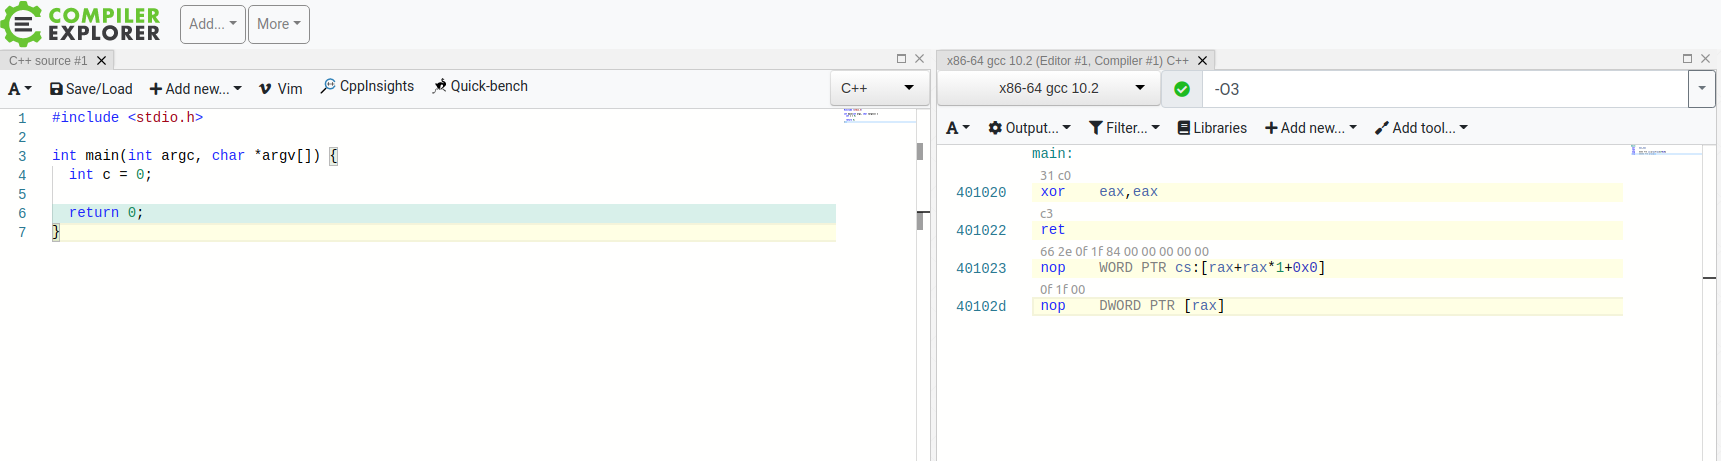
\includegraphics[width=1\linewidth]{imgs/chisel_after.png}
	\caption{\textbf{\texttt{C Code}} Example \color{green} after \color{black} \textbf{Chisel} tool processing}%
	\label{fig:plant}
\end{figure*}

\begin{table*}[]
	\centering
	\begin{tabular}{lccccccc}
		\hline
		\multicolumn{8}{c}{\textbf{NET UUID Program}}                                                                                                                                                                                                                                                                                                                                                                                                                                                                                                                                                                             \\ \hline
		\multicolumn{1}{l|}{\textbf{Libraries/Tools}}                                                                                  & \multicolumn{1}{c|}{\textbf{Before}} & \multicolumn{1}{c|}{\textbf{None}} & \multicolumn{1}{c|}{\textbf{Aggressive}} & \multicolumn{1}{c|}{{\color[HTML]{CB0000} \textbf{\begin{tabular}[c]{@{}c@{}}Machine  \\ Learning\end{tabular}}}} & \multicolumn{1}{c|}{\textbf{\begin{tabular}[c]{@{}c@{}}Non-rec \\ Aggressive\end{tabular}}} & \multicolumn{1}{c|}{\textbf{Only once}} & {\color[HTML]{32CB00} \textbf{\begin{tabular}[c]{@{}c@{}}IPDSE/IPSSCP\\ Loop Unrolling\end{tabular}}} \\ \hline
		\multicolumn{1}{l|}{{\color[HTML]{032F62} \textbf{Functions}}}                                                                 & 10                                   & 9                                  & 9                                        & 9                                                                                                                 & 9                                                                                           & 9                                       & 9                                                                                                     \\
		\multicolumn{1}{l|}{{\color[HTML]{032F62} \textbf{Basic Blocks}}}                                                              & 38                                   & 34                                 & 34                                       & 34                                                                                                                & 34                                                                                          & 34                                      & 34                                                                                                    \\
		\multicolumn{1}{l|}{{\color[HTML]{032F62} \textbf{Instructions Count}}}                                                        & 349                                  & 304                                & 304                                      & 304                                                                                                               & 304                                                                                         & 304                                     & 304                                                                                                   \\
		\multicolumn{1}{l|}{{\color[HTML]{032F62} \textbf{Direct Calls}}}                                                              & 23                                   & 20                                 & 20                                       & 20                                                                                                                & 20                                                                                          & 20                                      & 20                                                                                                    \\
		\multicolumn{1}{l|}{{\color[HTML]{032F62} \textbf{External Calls}}}                                                            & 12                                   & 9                                  & 9                                        & 9                                                                                                                 & 9                                                                                           & 9                                       & 9                                                                                                     \\
		\multicolumn{1}{c|}{{\color[HTML]{032F62} \textbf{\begin{tabular}[c]{@{}c@{}}Memory Instructions \\ Load/Store\end{tabular}}}} & 141                                  & 128                                & 128                                      & 128                                                                                                               & 128                                                                                         & 128                                     & 128                                                                                                   \\ \hline
	\end{tabular}
	\caption{Comparison of \texttt{DeepOCCAM} with other \texttt{OCCAM} Run settings and \texttt{OCCAM-T Run (Trimmer)}}
	\label{tab:my-table}
\end{table*}
\begin{table*}[]
	\centering
	\begin{tabular}{lccccccc}
		\hline
		\multicolumn{8}{c}{\textbf{netsh Program Program}}                                                                                                                                                                                                                                                                                                                                                                                                                                                                                                                                                                             \\ \hline
		\multicolumn{1}{l|}{\textbf{Libraries/Tools}}                                                                                  & \multicolumn{1}{c|}{\textbf{Before}} & \multicolumn{1}{c|}{\textbf{None}} & \multicolumn{1}{c|}{\textbf{Aggressive}} & \multicolumn{1}{c|}{{\color[HTML]{CB0000} \textbf{\begin{tabular}[c]{@{}c@{}}Machine  \\ Learning\end{tabular}}}} & \multicolumn{1}{c|}{\textbf{\begin{tabular}[c]{@{}c@{}}Non-rec \\ Aggressive\end{tabular}}} & \multicolumn{1}{c|}{\textbf{Only once}} & {\color[HTML]{32CB00} \textbf{\begin{tabular}[c]{@{}c@{}}IPDSE/IPSSCP\\ Loop Unrolling\end{tabular}}} \\ \hline
		\multicolumn{1}{l|}{{\color[HTML]{032F62} \textbf{Functions}}}                                                                 & 12                                   & 11                                 & 13                                       & 13                                                                                                                & 13                                                                                          & 11                                      & 11                                                                                                    \\
		\multicolumn{1}{l|}{{\color[HTML]{032F62} \textbf{Basic Blocks}}}                                                              & 313                                  & 312                                & 332                                      & 332                                                                                                               & 332                                                                                         & 312                                     & 312                                                                                                   \\
		\multicolumn{1}{l|}{{\color[HTML]{032F62} \textbf{Instructions Count}}}                                                        & 1319                                 & 1315                               & 1417                                     & 1417                                                                                                              & 1417                                                                                        & 1315                                    & 1315                                                                                                  \\
		\multicolumn{1}{l|}{{\color[HTML]{032F62} \textbf{Direct Calls}}}                                                              & 195                                  & 194                                & 196                                      & 196                                                                                                               & 196                                                                                         & 194                                     & 194                                                                                                   \\
		\multicolumn{1}{l|}{{\color[HTML]{032F62} \textbf{External Calls}}}                                                            & 172                                  & 171                                & 173                                      & 173                                                                                                               & 173                                                                                         & 171                                     & 171                                                                                                   \\
		\multicolumn{1}{c|}{{\color[HTML]{032F62} \textbf{\begin{tabular}[c]{@{}c@{}}Memory Instructions \\ Load/Store\end{tabular}}}} & 433                                  & 431                                & 481                                      & 481                                                                                                               & 481                                                                                         & 431                                     & 431                                                                                                   \\ \hline
	\end{tabular}
	\caption{Comparison of \texttt{DeepOCCAM} with other \texttt{OCCAM} Run settings and \texttt{OCCAM-T Run (Trimmer)}}
	\label{tab:my-table}
\end{table*}
\begin{table*}[]
	\centering
	\begin{tabular}{l|ll|ll|ll|ll|cl}
		\hline
		{\color[HTML]{3531FF} \textbf{Chisel Tool (Final)}}                                              & \multicolumn{2}{c|}{{\color[HTML]{000000} \textbf{bzip}}}                      & \multicolumn{2}{c|}{{\color[HTML]{000000} \textbf{date}}}                      & \multicolumn{2}{c|}{{\color[HTML]{000000} \textbf{mkdir}}}                     & \multicolumn{2}{c|}{{\color[HTML]{000000} \textbf{rm}}}                        & \multicolumn{2}{c}{{\color[HTML]{000000} \textbf{tree}}}                                           \\ \hline
		\textbf{Binary Metrics}                                                                          & {\color[HTML]{CB0000} \textbf{Before}} & {\color[HTML]{009901} \textbf{After}} & {\color[HTML]{CB0000} \textbf{Before}} & {\color[HTML]{009901} \textbf{After}} & {\color[HTML]{CB0000} \textbf{Before}} & {\color[HTML]{009901} \textbf{After}} & {\color[HTML]{CB0000} \textbf{Before}} & {\color[HTML]{009901} \textbf{After}} & \multicolumn{1}{l}{{\color[HTML]{CB0000} \textbf{Before}}} & {\color[HTML]{009901} \textbf{After}} \\ \hline
		\textbf{ROP Gadgets}                                                                             & 646                                    & 313                                   & 408                                    & 166                                   & 210                                    & 84                                    & 485                                    & 111                                   & 567                                                        & 405                                   \\
		\textbf{COP Gadgets}                                                                             & 97                                     & 55                                    & 39                                     & 8                                     & 7                                      & 5                                     & 44                                     & 5                                     & 50                                                         & 9                                     \\
		\textbf{JOP Gadgets}                                                                             & 6728                                   & 1562                                  & 5214                                   & 877                                   & 2282                                   & 176                                   & 4476                                   & 190                                   & 2126                                                       & 775                                   \\
		\textbf{\begin{tabular}[c]{@{}l@{}}Total Unique Gadgets\\ (Excluding SYS \& Chain)\end{tabular}} & 7374                                   & 1930                                  & 5626                                   & 1046                                  & 2492                                   & 260                                   & 4965                                   & 301                                   & 2693                                                       & 1187                                  \\ \hline
	\end{tabular}
	\caption{Dynamic Binary Analysis results for \texttt{Chisel} for \textbf{Gadgets Count}}
	\label{tab:my-table}
\end{table*}

\subsection{Comparision : Dynamic Analysis}%
\label{Tools}

Program debloating techniques. Program deblaoting techniques rogram debloating techniques. Program deblaoting techniques
rogram debloating techniques. Program deblaoting techniquesrogram debloating techniques. Program deblaoting techniques
rogram debloating techniques. Program deblaoting techniques rogram debloating techniques. Program deblaoting techniques
rogram debloating techniques. Program deblaoting techniques 
rogram debloating techniques. Program deblaoting techniquesrogram debloating techniques. Program deblaoting techniques
rogram debloating techniques. Program deblaoting techniques

Program debloating techniques. Program deblaoting techniques rogram debloating techniques. Program deblaoting techniques
rogram debloating techniques. Program deblaoting techniquesrogram debloating techniques. Program deblaoting techniques
rogram debloating techniques. Program deblaoting techniques rogram debloating techniques. Program deblaoting techniques
rogram debloating techniques. Program deblaoting techniques 
rogram debloating techniques. Program deblaoting techniquesrogram debloating techniques. Program deblaoting techniques
rogram debloating techniques. Program deblaoting techniques

\section{Observations}%
\label{Tools}

Program debloating techniques. Program deblaoting techniques rogram debloating techniques. Program deblaoting techniques
rogram debloating techniques. Program deblaoting techniquesrogram debloating techniques. Program deblaoting techniques
rogram debloating techniques. Program deblaoting techniques rogram debloating techniques. Program deblaoting techniques
rogram debloating techniques. Program deblaoting techniques 
rogram debloating techniques. Program deblaoting techniquesrogram debloating techniques. Program deblaoting techniques
rogram debloating techniques. Program deblaoting techniques

Program debloating techniques. Program deblaoting techniques rogram debloating techniques. Program deblaoting techniques
rogram debloating techniques. Program deblaoting techniquesrogram debloating techniques. Program deblaoting techniques
rogram debloating techniques. Program deblaoting techniques rogram debloating techniques. Program deblaoting techniques
rogram debloating techniques. Program deblaoting techniques 
rogram debloating techniques. Program deblaoting techniquesrogram debloating techniques. Program deblaoting techniques
rogram debloating techniques. Program deblaoting techniques

\subsection{Insights}%
\label{Tools}

Program debloating techniques. Program deblaoting techniques rogram debloating techniques. Program deblaoting techniques
rogram debloating techniques. Program deblaoting techniquesrogram debloating techniques. Program deblaoting techniques
rogram debloating techniques. Program deblaoting techniques rogram debloating techniques. Program deblaoting techniques
rogram debloating techniques. Program deblaoting techniques 
rogram debloating techniques. Program deblaoting techniquesrogram debloating techniques. Program deblaoting techniques
rogram debloating techniques. Program deblaoting techniques

Program debloating techniques. Program deblaoting techniques rogram debloating techniques. Program deblaoting techniques
rogram debloating techniques. Program deblaoting techniquesrogram debloating techniques. Program deblaoting techniques
rogram debloating techniques. Program deblaoting techniques rogram debloating techniques. Program deblaoting techniques
rogram debloating techniques. Program deblaoting techniques 
rogram debloating techniques. Program deblaoting techniquesrogram debloating techniques. Program deblaoting techniques
rogram debloating techniques. Program deblaoting techniques

\section{Conclusion}%
\label{Tools}

Program debloating techniques. Program deblaoting techniques rogram debloating techniques. Program deblaoting techniques
rogram debloating techniques. Program deblaoting techniquesrogram debloating techniques. Program deblaoting techniques
rogram debloating techniques. Program deblaoting techniques rogram debloating techniques. Program deblaoting techniques
rogram debloating techniques. Program deblaoting techniques 
rogram debloating techniques. Program deblaoting techniquesrogram debloating techniques. Program deblaoting techniques
rogram debloating techniques. Program deblaoting techniques

Program debloating techniques. Program deblaoting techniques rogram debloating techniques. Program deblaoting techniques
rogram debloating techniques. Program deblaoting techniquesrogram debloating techniques. Program deblaoting techniques
rogram debloating techniques. Program deblaoting techniques rogram debloating techniques. Program deblaoting techniques
rogram debloating techniques. Program deblaoting techniques 
rogram debloating techniques. Program deblaoting techniquesrogram debloating techniques. Program deblaoting techniques
rogram debloating techniques. Program deblaoting techniques

\subsection{But finally, Who Won?}%
\label{Tools}

Program debloating techniques. Program deblaoting techniques rogram debloating techniques. Program deblaoting techniques
rogram debloating techniques. Program deblaoting techniquesrogram debloating techniques. Program deblaoting techniques
rogram debloating techniques. Program deblaoting techniques rogram debloating techniques. Program deblaoting techniques
rogram debloating techniques. Program deblaoting techniques 
rogram debloating techniques. Program deblaoting techniquesrogram debloating techniques. Program deblaoting techniques
rogram debloating techniques. Program deblaoting techniques

Program debloating techniques. Program deblaoting techniques rogram debloating techniques. Program deblaoting techniques
rogram debloating techniques. Program deblaoting techniquesrogram debloating techniques. Program deblaoting techniques
rogram debloating techniques. Program deblaoting techniques rogram debloating techniques. Program deblaoting techniques
rogram debloating techniques. Program deblaoting techniques 
rogram debloating techniques. Program deblaoting techniquesrogram debloating techniques. Program deblaoting techniques
rogram debloating techniques. Program deblaoting techniques

\section{Other Tools}%
\label{Tools}

Program debloating techniques. Program deblaoting techniques rogram debloating techniques. Program deblaoting techniques
rogram debloating techniques. Program deblaoting techniquesrogram debloating techniques. Program deblaoting techniques
rogram debloating techniques. Program deblaoting techniques rogram debloating techniques. Program deblaoting techniques
rogram debloating techniques. Program deblaoting techniques 
rogram debloating techniques. Program deblaoting techniquesrogram debloating techniques. Program deblaoting techniques
rogram debloating techniques. Program deblaoting techniques

Program debloating techniques. Program deblaoting techniques rogram debloating techniques. Program deblaoting techniques
rogram debloating techniques. Program deblaoting techniquesrogram debloating techniques. Program deblaoting techniques
rogram debloating techniques. Program deblaoting techniques rogram debloating techniques. Program deblaoting techniques
rogram debloating techniques. Program deblaoting techniques 
rogram debloating techniques. Program deblaoting techniquesrogram debloating techniques. Program deblaoting techniques
rogram debloating techniques. Program deblaoting techniques

\section{Project Assets}%
\label{Tools}

Program debloating techniques. Program deblaoting techniques rogram debloating techniques. Program deblaoting techniques
rogram debloating techniques. Program deblaoting techniquesrogram debloating techniques. Program deblaoting techniques
rogram debloating techniques. Program deblaoting techniques rogram debloating techniques. Program deblaoting techniques
rogram debloating techniques. Program deblaoting techniques 
rogram debloating techniques. Program deblaoting techniquesrogram debloating techniques. Program deblaoting techniques
rogram debloating techniques. Program deblaoting techniques

Program debloating techniques. Program deblaoting techniques rogram debloating techniques. Program deblaoting techniques
rogram debloating techniques. Program deblaoting techniquesrogram debloating techniques. Program deblaoting techniques
rogram debloating techniques. Program deblaoting techniques rogram debloating techniques. Program deblaoting techniques
rogram debloating techniques. Program deblaoting techniques 
rogram debloating techniques. Program deblaoting techniquesrogram debloating techniques. Program deblaoting techniques
rogram debloating techniques. Program deblaoting techniques

\subsection{Docker Images}%
\label{Tools}

Program debloating techniques. Program deblaoting techniques rogram debloating techniques. Program deblaoting techniques
rogram debloating techniques. Program deblaoting techniquesrogram debloating techniques. Program deblaoting techniques
rogram debloating techniques. Program deblaoting techniques rogram debloating techniques. Program deblaoting techniques
rogram debloating techniques. Program deblaoting techniques 
rogram debloating techniques. Program deblaoting techniquesrogram debloating techniques. Program deblaoting techniques
rogram debloating techniques. Program deblaoting techniques

Program debloating techniques. Program deblaoting techniques rogram debloating techniques. Program deblaoting techniques
rogram debloating techniques. Program deblaoting techniquesrogram debloating techniques. Program deblaoting techniques
rogram debloating techniques. Program deblaoting techniques rogram debloating techniques. Program deblaoting techniques
rogram debloating techniques. Program deblaoting techniques 
rogram debloating techniques. Program deblaoting techniquesrogram debloating techniques. Program deblaoting techniques
rogram debloating techniques. Program deblaoting techniques

\subsection{GitHub Repositories}%
\label{Tools}

Program debloating techniques. Program deblaoting techniques rogram debloating techniques. Program deblaoting techniques
rogram debloating techniques. Program deblaoting techniquesrogram debloating techniques. Program deblaoting techniques
rogram debloating techniques. Program deblaoting techniques rogram debloating techniques. Program deblaoting techniques
rogram debloating techniques. Program deblaoting techniques 
rogram debloating techniques. Program deblaoting techniquesrogram debloating techniques. Program deblaoting techniques
rogram debloating techniques. Program deblaoting techniques

Program debloating techniques. Program deblaoting techniques rogram debloating techniques. Program deblaoting techniques
rogram debloating techniques. Program deblaoting techniquesrogram debloating techniques. Program deblaoting techniques
rogram debloating techniques. Program deblaoting techniques rogram debloating techniques. Program deblaoting techniques
rogram debloating techniques. Program deblaoting techniques 
rogram debloating techniques. Program deblaoting techniquesrogram debloating techniques. Program deblaoting techniques
rogram debloating techniques. Program deblaoting techniques

\nocite{*}
\begin{thebibliography}{9}
	\bibitem{latexcompanion} 
	Michel Goossens, Frank Mittelbach, and Alexander Samarin. 
	\textit{The \LaTeX\ Companion}. 
	Addison-Wesley, Reading, Massachusetts, 1993.
	
\end{thebibliography}
\end{document}

